\section{Architectural Design}

The purpose of this section is to present and analyze the architecture of the software to be system in a top-down manner. We first introduced the overall architecture and then provided a diagram of the system’s components, focusing on the tournaments and battles sub-components. Next, we used an ER diagram to describe the system’s logical data and presented the system’s deployment view, including the layers and tiers involved. We also used sequence diagrams to depict important runtime views and class diagrams to analyze the component interfaces. Finally, we discussed the architectural design choices and the reasons behind them.

\subsection{Overview}
The figure shown below represents a high-level description of the components which make up the System.
It is a distributed system with a 4-tier architecture: presentation, web server, application server and database. In this document, the presentation layer and the Client will be referred to as the Frontend, while the Application Layer and the Data Layer will be referred to as the Backend.
\\
\begin{figure}[h]
    \center
    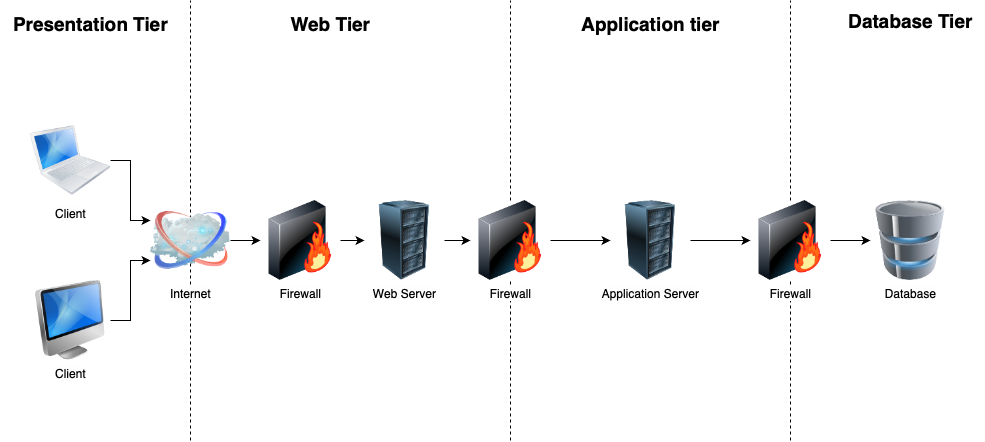
\includegraphics[width=1\linewidth]{src/High level system architecture.png}
    \caption{High level system architecture}
    \label{fig:High level system architecture}
\end{figure}
\\
The presentation tier is the client side, where users interact with the system through a web browser. A single page application will be developed both for educators and students to use the system. The reason behind this choice is the ease of interaction without the need for frequent page reloading, providing a better user experience.\\
The web server is responsible for communication between the Frontend and the Backend. It handles HTTP requests, routing them to the appropriate components. It supports secure communication with clients through HTTPS, and load balancing ensures optimal performance during periods of high traffic.\\
The application tier is the logic core of our system. It processes data received from the presentation tier, performs business logic operations, and communicates with the database. It tier ensures data integrity, security, and authentication, with role-based access controls. It interfaces with external services or APIs as needed. \\
Finally, the data tier is responsible for storing, reading and updating all information necessary for the system. We use a relational database that offers high scalability potential for structured data.
It interfaces with the application tier, granting data access and manipulation while respecting security protocols.\\
The client web-server and web-server application-server communication use HTTP, while app-server DBMS communication relies on APIs. The app-servers are designed to be stateless according to REST standards. The system also includes firewalls to enhance security.\\

\subsection{Component view}
In this section we offer a more detailed view of the S2B. We will focus on the components and their interactions, along with the interfaces. To meet performance and availability criteria, most of said components will be duplicated or replicated.
\begin{figure}[h]
    \centering
    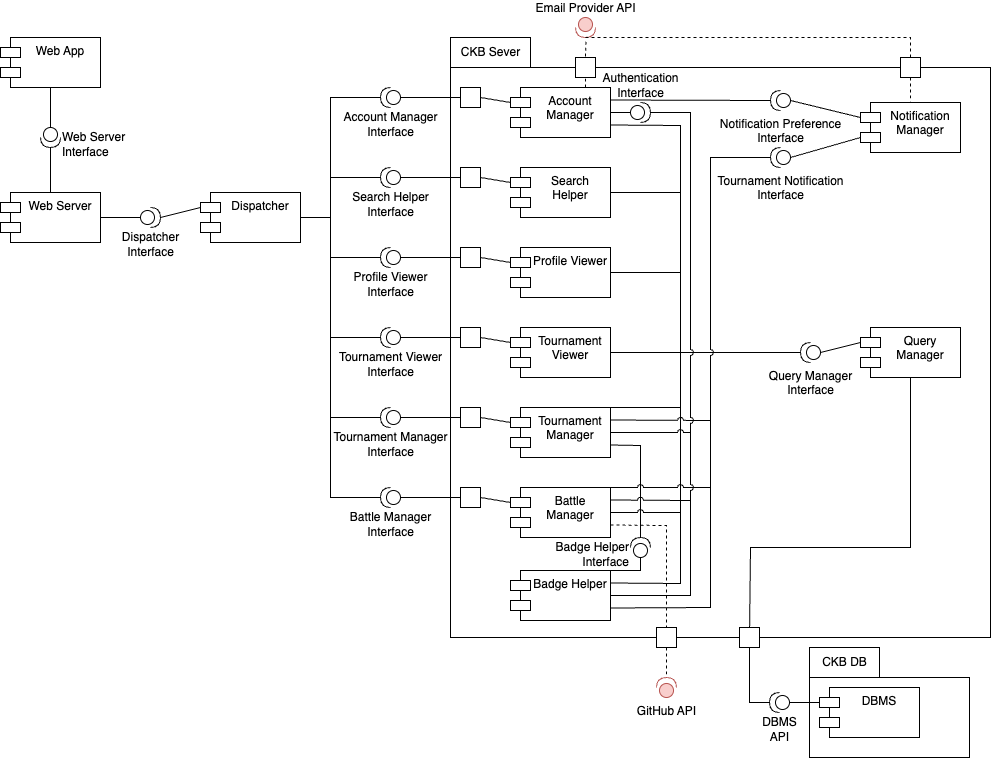
\includegraphics[width=1\linewidth]{src/Component Diagram of the CKB System.png}
    \caption{Component Diagram of the CKB System}
    \label{fig:Component Diagram of the CKB System}
\end{figure}
\\
\\
\\
\begin{itemize}
    \item \textbf{Web server}\\
    The web server is designed to handle HTTP requests from the client, redirecting them to the appropriate components. It uses client-side rendering. As the user interacts with the page, further requests may be automatically made and the page will be updated dynamically without requiring a full page reload.\\
    \item \textbf{CKB server}\\
    The CKB server is responsible for the business logic and provide the full functionality to users. Since most of the functionalities offered are shared between educators and students, there will not be a different server for each user category. It is further composed of different components.\\
    \begin{itemize}
        \item \textbf{CKB’s Account Manager}\\
        This component handles all the account operations related to the users and offers an interface to authenticate the requests. It offers functionality to create new account, logging in, setting preferences and verify the authentication of the user at any time. To create a new account, It interacts with the external email provider API to make the user receive a code to verify the identity.\\
        \item \textbf{Search helper}\\
        This component enables the search functionality, letting users and non-users search for a specific user or a specific tournament. It also allows filtering based on date posted, number of awards, ongoing/finished, number of participants and much more (tournaments).\\
        \item \textbf{Profile viewer}\\
        This component allows viewing profiles of users subscribed to CKB, both educators and students. Anyone can see profiles, even unsubscribed users. Within the profile page, there may be tournaments the user took part in (as a student or as an educator) and clicking them will redirect that tournament page.\\
        \item \textbf{Tournament viewer}\\
        This component allows viewing tournaments, along with the battle pages in the scope of It. Anyone can see tournaments, even unsubscribed users. You can find all the information related to that tournament, as well as the battles, including teams, final rank for each battle and much more.\\
        \item \textbf{Tournament manager}\\
        This component allows managing and creating tournaments for educators and subscribing to them for students. The creator can grant other educators permission to create battles. For ongoing tournaments, allowed educators can create new battle clicking the right button. Such functionality is provided through the next component.\\
        \item \textbf{Battle manager}\\
        This component allows managing and creating battles for educators and joining them for students. It also manages the team functionality, allowing students to team up for each battle. \\
        \item \textbf{Badge helper}\\
        This component enables the gamification aspects of CKB. It allows educators to create badges and define new rules as well as new variables associated with them. Badges are then linked to the profile of users achieving them, making them visible to anyone.\\
        \item \textbf{CKB Notification Service}\\
        This component enables the CKB notifications. Users will receive notifications about important events, like new tournaments created, tournament to which the user is subscribed closes and more.
        \newline
        \newline
        \textbf{External APIs}\\
        \item \textbf{GitHub API}\\
        This API enables the GitHub integration: new repositories automatically created (e.g. when a new battle begins) and sources automatically downloaded (e.g. when a user pushes new code to the main branch of his repository)\\
        \item \textbf{Email provider API}
        This service is used for authentication during registration and for important notifications.
    \end{itemize}
    \vspace{1cm}
    \item \textbf{Query Manager}
    \\This component is responsible for communicating with the Database Management System. It follows the adapter pattern, allowing  easier communication between other components and the DBMS.
\end{itemize}

\vspace{1cm}

\subsection{Deployment view}
This chapter describes the deployment of the system.
\begin{figure}[h]
    \centering
    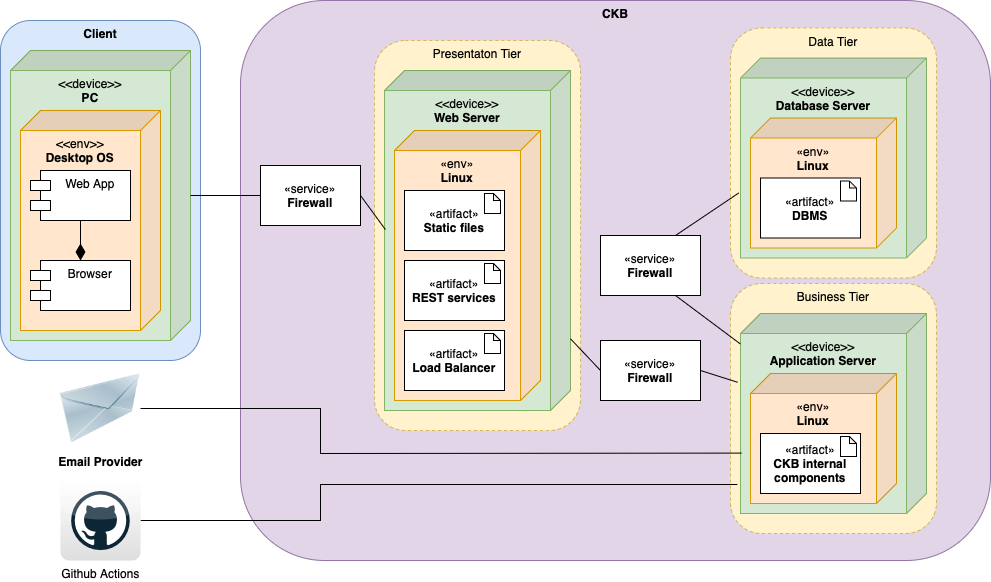
\includegraphics[width=1\linewidth]{src/Deployment View of the system.png}
    \caption{Deployment View of the system}
    \label{fig:Deployment View of the system}
\end{figure}
\\
\begin{itemize}
    \item \textbf{Web-server}\\
    The web-server will be the entry point for the SPA. It forwards the requests to the application-server. A modern device with access to a web browser is required to interface with the web-server. 
    \item \textbf{Load Balancer}\\
    This device is responsible for load balancing, which means, distributing incoming network traffic and requests across multiple servers. Its primary purpose is to optimise resource utilization, enhance reliability while ensuring high availability.
    \item \textbf{Firewall}\\
    Firewalls are used to filter connections to the application and data layers of a system. They are located between the internet and the system intranet. They offer additional security blocking or allowing traffic based on predetermined rules.
\end{itemize}

\subsection{Runtime View}
This section illustrates the interactions between actors, subsystems and interfaces of the system showing the specific method called.

\subsection{Component Interfaces}
This section lists all the methods offered by each component interface to the other components.

\subsection{Selected architectural styles and patterns}
\begin{itemize}
    \item \textbf{Three layer four tier}\\
    This architecture offers several benefits. It allows the distinction of layers (presentation, logic, data) and tiers (client, web server, application server, DBMS), which makes the system more modular and easier to maintain. Such separation also allows better scalability and better workload distribution across multiple servers. Finally, load balancing and caching techniques are available to further increase performance and availability.

    \item \textbf{RESTful APIs}\\
    The API is based on standard web technologies, like JSON or XML, allowing better integration with other systems. It is stateless, which makes the development easier. It also promotes simplicity and scalability.\\
    \item \textbf{Adapter pattern}\\
    The Adapter Pattern seamlessly integrates different components, standardizing interfaces and ensuring flexibility. It hides the underlying complexity and provides a set of high-level functions. 
\end{itemize}

\vspace{1cm}
    
\subsection{Other design decisions}
\begin{itemize}
    \item SQL database
    SQL databases offer high scalability and decent performance for structured data. It follows ACID principles and ensures data integrity. Overall, It is a good compromise for performance, consistency, reliability and ease of use.
\end{itemize}